\documentclass{article}
\usepackage{amsmath, amssymb, amsthm, enumitem,fullpage,tikz,microtype,polynom,placeins,forest}
\usepackage{docmute}
\newtheorem{corollary}{Corollary}
\newtheorem{lemma}{Lemma}
\usetikzlibrary{trees}

\title{Catalan Numbers}
\author{Tomasz Brengos \\  
Committers : Aliaksei Kudzelka}
\date{}

\begin{document}
\maketitle
\section{Introduction and Motivating Problem}

How many ways can we correctly place $n$ pairs of parentheses? This is a classic combinatorial question about **valid parentheses combinations**. For example, with $n=1$ pair, there is only one valid arrangement: `()`. With $n=2$ pairs, there are two valid arrangements: `()()` and `(())`. With $n=3$ pairs, there are five valid arrangements (e.g. `()()()`, `()(())`, `(())()`, `(()())`, `((()))`). In general, the number of distinct well-formed parentheses sequences grows quickly with $n$. 

This problem was our motivation to study a famous sequence of numbers. (It has connection to a similar LeetCode programming problem about generating parentheses.) The numbers counting valid parentheses structures for $n=1,2,3,\dots$ are:

\[1,\; 2,\; 5,\; 14,\; 42,\; 132,\;\dots\]

These are known as the **Catalan numbers**. In these notes, we will explore Catalan numbers, their recursive definition, how they relate to binary tree structures, and a derivation of their formula using generating functions.

\section{Definition of Catalan Numbers}

The Catalan numbers $C_n$ can be defined recursively. For $n=0$ (zero pairs of parentheses), we define $C_0 = 1$ by convention (there is exactly one valid arrangement of zero pairs: an empty sequence). For $n\ge 1$, the Catalan number $C_n$ satisfies the recursion:

\[
C_n \;=\; \sum_{k=0}^{\,n-1} C_k \;\cdot\; C_{\,n-1-k}\,.
\]

In other words, each $C_n$ is obtained by summing over all products $C_k \cdot C_{n-1-k}$ for $0 \le k \le n-1$. This recurrence is the heart of what makes Catalan numbers arise in so many combinatorial structures. We will soon see why this recurrence formula makes sense in terms of counting valid parentheses or binary tree configurations.

\textit{*(Additional note: There is also a direct formula for $C_n$ which we will derive later. The first few values $C_0=1$, $C_1=1$, $C_2=2$, $C_3=5$, $C_4=14$ confirm the sequence given above.)*}

\subsection*{Combinatorial reasoning (parenthesis perspective)}

Why does the above recurrence hold for valid parentheses? Consider a valid parentheses sequence of $n$ pairs. Focus on the very first “(`” character. It must have a matching “)`”. Say this matching “)`” occurs after forming $k$ pairs inside (between this “(`” and its matching “)`”) – those $k$ pairs inside must themselves form a valid sequence. The remaining parentheses (after the matching “)`”) will form another valid sequence with $n-1-k$ pairs. See the schematic below for a sequence split by the first pair:

\[
\underbrace{\vphantom{()}( \;\;\; S_{\text{inside}} \;\;\; )}_{\text{$1+k$ pairs}} \;\; S_{\text{outside}}\,,
\] 

where $S_{\text{inside}}$ is a valid sequence of $k$ pairs, and $S_{\text{outside}}$ is a valid sequence of $n-1-k$ pairs. Any valid sequence can be uniquely decomposed in this way. There are $C_k$ possibilities for $S_{\text{inside}}$ and $C_{\,n-1-k}$ possibilities for $S_{\text{outside}}$. Multiplying and summing over all $k$ from $0$ to $n-1$ gives the recurrence $C_n = \sum_{k=0}^{n-1} C_k\,C_{n-1-k}$, as stated above.

\textit{*(Additional note: The same recurrence will be explained again using binary trees below, which is an equivalent interpretation. The key idea is splitting a structure (parentheses or tree) at a certain point, resulting in two smaller independent structures.)*}

\section{Catalan Numbers and Binary Trees}

Catalan numbers also count the number of distinct **binary tree** structures with a given number of nodes. To appreciate this connection, we first review what a binary tree is:

A **binary tree** is a hierarchical structure consisting of nodes, where each node may have up to two children: a left child and a right child. A node with no children is called a *leaf*. We often draw binary trees in a planar way with the root at the top, left children branching to the left, and right children to the right. In counting binary trees for Catalan numbers, we consider different shapes of the tree (different arrangements of nodes and child connections) as distinct, but we do *not* label the nodes with any specific values.

For example, with only 1 node, there is exactly one possible binary tree (just the root by itself). With 2 nodes, there are exactly two distinct binary tree shapes:

\begin{center}
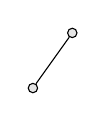
\begin{tikzpicture}[level distance=7mm, sibling distance=10mm, every node/.style={circle, draw, fill=black!10, inner sep=1.2pt}]
\node {} 
  child { node {} }
  child[missing] {};
\end{tikzpicture}
\hspace{1cm}
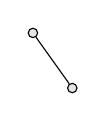
\begin{tikzpicture}[level distance=7mm, sibling distance=10mm, every node/.style={circle, draw, fill=black!10, inner sep=1.2pt}]
\node {}
  child[missing] {} 
  child { node {} };
\end{tikzpicture}
\end{center}

In the first tree above, the root has a left child but no right child. In the second tree, the root has a right child but no left child. These are the only two possible configurations for 2 nodes. Now, for 3 nodes, it turns out there are 5 distinct binary tree shapes. We can enumerate all five (to visualize them, each diagram below shows the shape, with nodes represented by circles):

\begin{center}
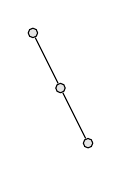
\begin{tikzpicture}[baseline=-2pt, level distance=7mm, sibling distance=7mm, every node/.style={circle, draw, fill=black!10, inner sep=1.2pt}]
\node {} 
  child[missing] {} 
  child { node {} 
            child[missing] {} 
            child { node {} } };
\end{tikzpicture}
\hfill
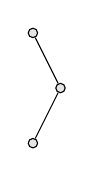
\begin{tikzpicture}[baseline=-2pt, level distance=7mm, sibling distance=7mm, every node/.style={circle, draw, fill=black!10, inner sep=1.2pt}]
\node {}
  child[missing] {} 
  child { node {}
            child { node {} } 
            child[missing] {} };
\end{tikzpicture}
\hfill
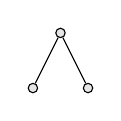
\begin{tikzpicture}[baseline=-2pt, level distance=7mm, sibling distance=7mm, every node/.style={circle, draw, fill=black!10, inner sep=1.2pt}]
\node {} 
  child { node {} }
  child { node {} };
\end{tikzpicture}
\hfill
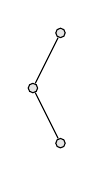
\begin{tikzpicture}[baseline=-2pt, level distance=7mm, sibling distance=7mm, every node/.style={circle, draw, fill=black!10, inner sep=1.2pt}]
\node {}
  child { node {}
            child[missing] {} 
            child { node {} } }
  child[missing] {};
\end{tikzpicture}
\hfill
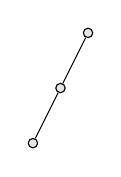
\begin{tikzpicture}[baseline=-2pt, level distance=7mm, sibling distance=7mm, every node/.style={circle, draw, fill=black!10, inner sep=1.2pt}]
\node {}
  child { node {}
            child { node {} } 
            child[missing] {} }
  child[missing] {};
\end{tikzpicture}
\end{center}

\vspace{1ex}
\begin{center}
\small (All 5 distinct binary trees with 3 nodes)
\end{center}
\vspace{1ex}

For 3 nodes, the five tree shapes can be described as:
1. A right-skewed chain (root $\to$ right child $\to$ right grandchild).
2. A tree where the root has only a right child, and that child in turn has a left child.
3. A balanced tree (root with one left child and one right child).
4. A tree where the root has only a left child, and that child has a right child.
5. A left-skewed chain (root $\to$ left child $\to$ left grandchild).

If we proceed to 4 nodes, the number of distinct binary trees grows to 14. Detailing all 14 shapes is cumbersome, but we can categorize them by how the root splits the nodes between left and right subtrees:
- 5 of those trees have all 3 of the other nodes in the left subtree (and right subtree empty), and another 5 have all 3 in the right subtree (left empty). These 10 are essentially a root with one side empty and the other side being one of the 5 shapes from the 3-node case.
- 2 of the trees have the root with 1 node in the left subtree and 2 in the right subtree.
- The remaining 2 have 2 nodes in the left subtree and 1 in the right subtree.

Adding these cases: $5 + 5 + 2 + 2 = 14$ total shapes for 4 nodes. (Indeed, 14 is the next Catalan number after 5.)

This pattern is no coincidence. In fact, the recurrence relation for $C_n$ can be understood by considering how a binary tree of $n$ nodes can be formed. Suppose a binary tree has $n$ nodes in total. Pick a number $k$ between $0$ and $n-1$ (inclusive) to be the number of nodes in the left subtree of the root. Then the right subtree will have $n-1-k$ nodes (since one node is the root itself). There are $C_k$ possible shapes for the left subtree (by definition of Catalan numbers for $k$ nodes) and $C_{\,n-1-k}$ possible shapes for the right subtree. These choices are independent, so there are $C_k \cdot C_{\,n-1-k}$ possible trees with that particular split of $k$ and $n-1-k$. Summing over all $k=0,1,2,\dots,n-1$ gives exactly $C_n = \sum_{k=0}^{n-1} C_k\,C_{n-1-k}$. This is the same recursive formula we encountered earlier, now interpreted in terms of binary trees. Thus, the number of valid parentheses arrangements with $n$ pairs is equal to the number of binary tree structures with $n$ nodes, and both are given by the $n$th Catalan number.

\section{Deriving the Formula using Generating Functions}

While the recursive definition of Catalan numbers is useful, we can go further and derive a closed-form formula for $C_n$. A powerful method to solve such recurrences is to use a **generating function**. Define the generating function $C(x)$ for the Catalan sequence as:

\[
C(x) \;=\; C_0 + C_1 x + C_2 x^2 + C_3 x^3 + \cdots \;=\; \sum_{n\ge 0} C_n \, x^n\,.
\]

Using the recurrence $C_n = \sum_{k=0}^{n-1} C_k\,C_{n-1-k}$, we can derive an equation for $C(x)$. First, note that:

\[
C(x) - C_0 \;=\; \sum_{n\ge 1} C_n x^n \;=\; \sum_{n\ge 1}\Big(\sum_{k=0}^{n-1} C_k\,C_{n-1-k}\Big) x^n\,.
\]

Now, change the summation index by letting $m = n-1$. Then $n\ge 1$ corresponds to $m \ge 0$, and $n = m+1$. The above becomes:

\[
C(x) - 1 \;=\; \sum_{m\ge 0} \Big(\sum_{k=0}^{m} C_k\,C_{m-k}\Big) x^{\,m+1} \;=\; x \sum_{m\ge 0} \sum_{k=0}^{m} C_k\,C_{m-k}\; x^m\,.
\]

But the double sum $\sum_{m\ge 0}\sum_{k=0}^{m} C_k C_{m-k} x^m$ is recognized as the product of two power series. In fact, by the Cauchy convolution formula, 

\[
\sum_{m\ge 0}\sum_{k=0}^{m} C_k\,C_{m-k}\; x^m \;=\; \Big(\sum_{k\ge 0} C_k x^k\Big)\Big(\sum_{j\ge 0} C_j x^j\Big) \;=\; C(x)\,C(x) \;=\; [C(x)]^2\,.
\]

Therefore, we have the following functional equation for $C(x)$:

\[
C(x) - 1 \;=\; x\,[C(x)]^2\,,
\] 

or equivalently,

\[
C(x) \;=\; 1 \;+\; x\,[C(x)]^2\,.
\]

This equation is derived directly from the Catalan recurrence. Now we solve for $C(x)$ as an explicit function of $x$. The equation $C(x) = 1 + x[C(x)]^2$ can be rearranged into a quadratic equation in $C(x)$:

\[
x [C(x)]^2 - C(x) + 1 = 0\,.
\]

Solving this quadratic for $C(x)$, we use the quadratic formula (treating $C(x)$ as the unknown and $x$ as a constant):

\[
C(x) \;=\; \frac{1 \pm \sqrt{\,1 - 4x\,}}{2x}\,. 
\]

There are two solutions, but we must choose the one that gives a valid power series expansion. Since $C(0)$ should equal $C_0 = 1$, we take the **negative** branch of the $\pm$ (this ensures $C(x)$ is finite at $x=0$):

\[
C(x) \;=\; \frac{\,1 - \sqrt{\,1 - 4x\,}\,}{2x}\,.
\]

This is the generating function for the Catalan numbers. We can expand this to obtain a formula for $C_n$. The series expansion of the square root can be derived using the binomial series:

\[
\sqrt{\,1 - 4x\,} \;=\; 1 \;-\; 2x \;-\; 2x^2 \;-\; 4x^3 \;-\; 8x^4 \;-\; \cdots\,,
\] 

but a more straightforward way is to recognize the known power series for Catalan numbers. In fact, the coefficient extraction can be done by comparing with the binomial theorem. The final result (which one can derive by expanding or by known combinatorial identities) is:

\[
C_n \;=\; \frac{1}{\,n+1\,}\binom{2n}{\,n}\,,
\] 

for $n \ge 0$. This elegant formula gives the $n$th Catalan number directly. For example, for $n=4$ it gives $C_4 = \frac{1}{5}\binom{8}{4} = \frac{1}{5}\cdot 70 = 14$, consistent with our earlier count of binary trees or parentheses combinations.

\textit{*(Additional note: The closed-form formula above was not explicitly given in the lecture, but it is a well-known result for Catalan numbers. It can be proven by induction or other methods as well. Catalan numbers appear in numerous other combinatorial problems, such as counting paths in a grid, polygon triangulations, full binary trees with $n+1$ leaves, and many more.)*}


\end{document}